% -*-LaTeX-*-

% The log below is the old log from when RCS was being used in
% conjunction with this.
%
% $Log: computer-signals.tex,v $
% Revision 1.8  2010/03/16 00:26:08  stiber
% Minor clarification.
%
% Revision 1.7  2007/12/25 17:46:12  stiber
% Some final cosmetic changes.
%
% Revision 1.6  2007/12/08 17:22:10  stiber
% Minor edits and corrections for Winter 2008.
%
% Revision 1.5  2007/03/20 23:52:12  stiber
% Cleaned up and updated LaTeX.
%
% Revision 1.4  2007/03/10 19:25:06  stiber
% Updated chapter for stand-alone textbook. Incorporated suggestions
% from Donald Christopherson.
%
% Revision 1.3  2006/03/27 23:35:14  stiber
% Fixed mistakes in end-of-chapter problem.
%
% Revision 1.2  2004/03/29 19:51:15  stiber
% Updated for Spring 2004 and new textbook (DSP First).
%
% Revision 1.1  2004/02/19 00:23:17  stiber
% Initial revision
%

\chapter{Signals in the Computer}
\label{ch:computer-signals}

In chapter~\ref{ch:physical-signals}, you were introduced to the
nature of physical signals and how they can be described
mathematically.  In this chapter, we move onward to discuss how these
``real world,'' analog signals end up inside computers: analog to
digital conversion (A/D conversion, or ADC). We then develop the first
little bit of a fundamental mathematical representation of such
\emph{discrete} signals. In the process, we visit the problems that
digitization creates. At the end of this chapter, you should have a
basic grasp of how ADC works and the tradeoffs involved in A/D
parameters versus the characteristics of the analog signal.

\section{From the physical to the digital}

Physical signals fundamentally involve application of energy to cause
some physical quantity to change. For instance, sound is carried by
waves of changing air pressure; images are patterns of emitted and/or
reflected light. On the other hand, computer signals are collections
of binary numbers --- vectors for sound, 2D arrays for images, or
sequences of 2D arrays for video. The process of bridging this gap is
the process of connecting the analog world to the digital
computer, or \emph{data acquisition}. There are three parts to this
\index{data acquisition}
process:
\begin{enumerate}
\item transduction,
\item sampling, and
\item quantization.
\end{enumerate}

\begin{figure}
\centerline{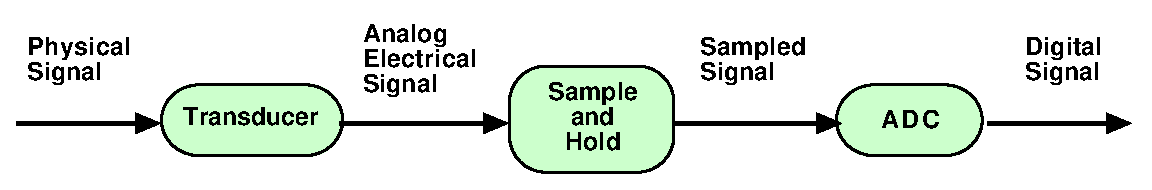
\includegraphics[width=\textwidth]{ch-computer/adc}}
\caption{Block diagram of the data acquisition process.\label{fg:adc}}
\end{figure}

Figure~\ref{fg:adc} shows these three steps and the intervening
representations of the signal.  This is an important point: the
``real'' signal is the physical one; what we seek to do is to produce
a \emph{representation} of this signal within the computer. Our goal
is that this representation will carry all the information of interest
that the original had. In this chapter, we will concern ourselves primarily
with two ways that information (fidelity) is destroyed: sampling and
quantization.

But, before either can be performed, the physical signal must be
converted into an analog, electrical signal. This process, known as
\emph{transduction}, involves a sensor that responds to the physical
\index{transduction} signal and produces an electrical output. A
microphone is such a sensor: it might include a membrane that vibrates
in response to air pressure changes which in turn moves a coil of wire
around a magnet to produce an electric current in the coil. Image
sensors are typically composed of 2D arrays of charge-coupled devices
(CCDs), in which photons affect the leakage of electrical charge. A
sensor is typically connected to signal conditioning hardware (not
shown), which amplifies its output to match the subsequent stages'
inputs and may perform filtering operations (we'll discuss this
filtering later in the chapter).  The result of transduction is truly
an analog signal: it is an electrical waveform whose value is
proportional to the physical signal. Herein lies our first source of
\emph{noise}.

Transduction always results in noise. Temperature variations, humidity
conditions, and a variety of other sources cause the sensor
representation of a signal to be imperfect. In a microphone, the
relationship between the sensor output and the actual sound may be
non-linear, or there may static noise from other devices (i.e., a hum
in the background). For cameras, low light conditions can cause
graininess, a random fluctuation of the actual signal. However, noise
can be introduced in many parts of the digitization process.

\index{analog-to-digital conversion|(}
\index{digitization|see{analog-to-digital conversion}}
Figure~\ref{fg:adc} also presents the basic process of digitization
--- converting an analog electrical signal into a sequence of binary
numbers.  Digitization involves two processes: \emph{sampling} and
\emph{quantization}.  In the former process, the value of the analog
signal is measured at regular intervals of time (the \emph{sampling
interval}). The output of a sample and hold (S/H) device will
maintain a fixed level in between sampling times. This makes the
quantization process easier: the analog-to-digital converter (ADC)
takes an analog signal at some fixed voltage (the sampled signal) and
produces a binary output that approximates the voltage ---
quantization. Each of these processes, together with transduction, will add noise to the signal in one form or another. It is important to know how to measure this noise and how to avoid it at each step. 

\section{Measuring Noise}
The fidelity of a signal is defined as the correspondence between an
input signal and an output signal. A signal with high distortion has
low fidelity. We will need to define three terms in order to measure
the amount to which a signal is distorted:
\begin{enumerate}
\item Root mean square (RMS) magnitude: this defines the ``power''
  that a signal has. For a signal $f(t)$ with a period of $T$ we
  define the RMS magnitude as
  $f_\mathrm{RMS}=\sqrt{\frac{1}{T}\int_{T}f(t)^2 dt}$. Where $\int_T$
  denotes that the integral is taken over one period of
  $f(t)$. Intuitively, a signal with large values will also have a
  large RMS magnitude.
\item Signal-to-noise ratio (SNR): this compares the RMS magnitude of
  the signal, $x_\mathrm{RMS}$, to the RMS magnitude of the noise,
  $n_\mathrm{RMS}$. SNR is defined as
  $x_\mathrm{RMS}/n_\mathrm{RMS}$. The noise signal, $n(t)$, can be
  measured directly (taking the difference between the noisy signal
  and the reference signal, if available) or indirectly (such as using
  the expected noise magnitude for a given application or device).
\item The decibel (dB): we normally convert SNR into a dB scale using
  $\text{SNR}_\mathrm{dB}=20\log_{10}(\text{SNR})$. There are
  historical and perceptual reasons for using the decibel scale, but,
  practically, it helps to compare large and small SNR values on the
  same graph. The log operation makes very small SNR values large
  negative numbers and simultaneously makes very large SNR values
  lesser in magnitude.
\end{enumerate}
\index{signal-to-noise ratio (SNR)}
\index{decibel}
Mathematically, SNR becomes:
\begin{equation}
\text{SNR}=20\log_{10}\left(\frac{x_\mathrm{RMS}}{n_\mathrm{RMS}}\right) \label{eq:SNR}
\end{equation}
We can quantify the amount of noise in a signal by using the SNR. The
idea is that noise becomes more of a problem when it reaches the same
magnitude as the signal. For example, a slight hissing noise on a
loudspeaker is not as troublesome as the same hissing noise in a
telephone conversation because the signal from the loudspeaker
``overpowers'' the noise signal. At each stage of transduction and
digitization, we can use SNR to tell us exactly how much distortion we
have introduced into the signal. There are other measures of fidelity
of a signal (actually it is an open research problem in many fields),
however, we will concentrate on SNR because it is the most widely used
measure and is not specific to any application.

\section{Sampling}

\begin{figure}
\centerline{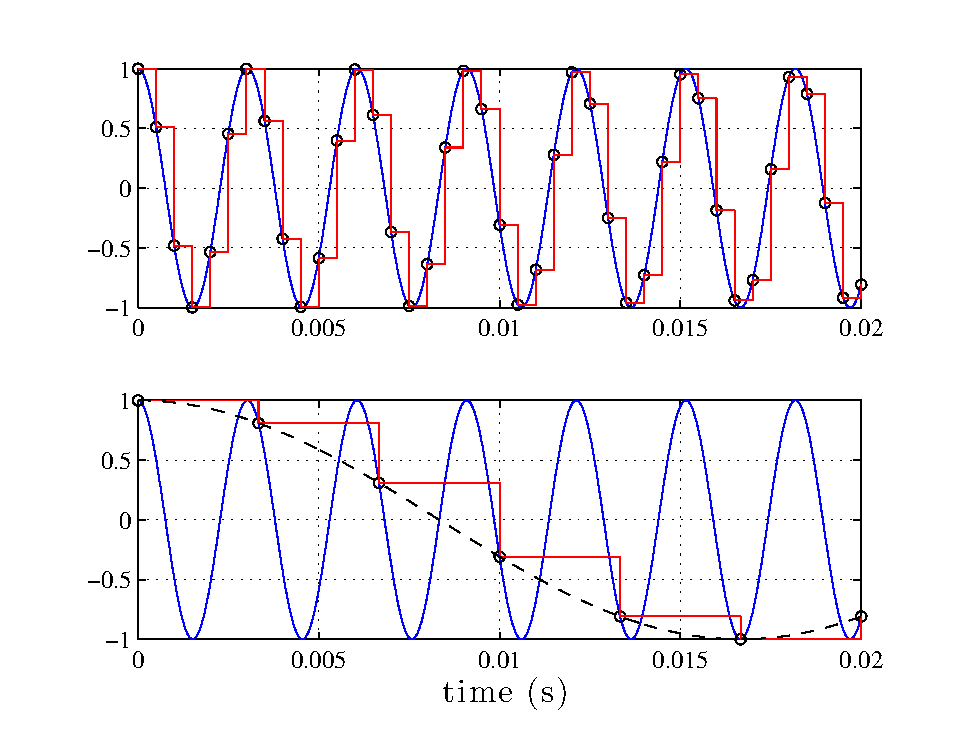
\includegraphics[width=\textwidth]{ch-computer/sampled}}
\caption[Sample and hold output]{Sample and hold
output. Analog input signal (sinusoidal curve) is a 330Hz sine wave; sampling
rate is 2000Hz (top) and 300 Hz (bottom). Output of S/H is red lines. Discrete value are shown as dark circles.\label{fg:sampled}}
\end{figure}

\index{analog-to-digital conversion!sampling|(} A sample and hold
(S/H) device acts like a switch and an analog memory device. While we
may talk of sampling a signal at a \emph{point} in time, a real device
requires a \emph{period} of time to perform its function, and this
includes sampling.  Over some short period of time, the S/H closes its
``switch'' and the analog signal is presented to the memory device
(which can be considered to be a capacitor, for example). The memory
device's internal voltage takes a short time to reach equilibrium with
the applied voltage --- called the \emph{aperture time}. After this
aperture time, the ``switch'' is opened and the sampled signal stays
stable while the ADC converts the signal to a digital value. However,
the sampled signal doesn't stay perfectly constant --- some of the
stored electrical charge leaks away, and thus the sampled signal
``sags'' towards zero volts.  While these limitations of the physical
device are important for sensor design and de-noising, we will focus
on the basic idea of sampling at points in time and assume the S/H
performs like an ideal device. Figure~\ref{fg:sampled} shows the
input/output behavior of such an idealized device.

%\begin{figure}
%\centerline{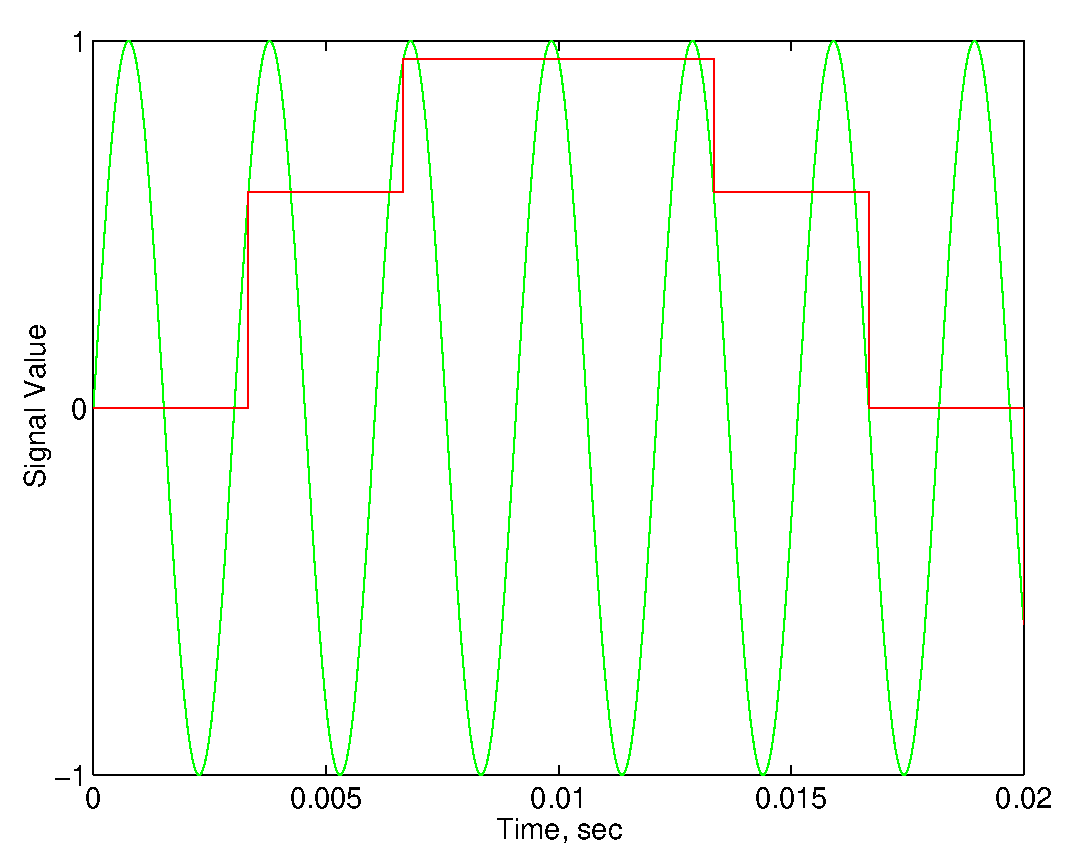
\includegraphics[width=\textwidth]{ch-computer/sampled_300}}
%\caption[Sample and hold output; 300Hzsampling rate]{Sample and hold
%output. Analog input signal (green) is a 330Hz sine wave; sampling
%rate is 300Hz. Output of S/H is plotted in red.\label{fg:sampled300}}
%\end{figure}

\index{Nyquist limit|see{analog-to-digital conversion, aliasing}}
\index{analog-to-digital conversion!aliasing|(}
We've already stated that we'd like the digitization process to retain
all the information in the original physical signal (or, at least,
that not being possible, to retain all information as far as is practical).
However, sampling alone can destroy information. In the case of
figure~\ref{fg:sampled} (top), no information is lost (the original
waveform could in principle be reconstructed) because the sampling
rate, at 2000Hz, is much higher than the sinusoid's frequency, 330Hz.
Of course, the higher the sampling rate the more expensive the S/H and
ADC, and the more data produced at the output (i.e., a
higher data rate).  How slowly can we sample a sinusoid?
Figure~\ref{fg:sampled} (bottom) shows the same sinusoid, but this time sampled at 300Hz. In the 20ms
plotted, the original signal goes through approximately six cycles. If
we look at the sampled signal, it looks like a sampled version of a
sinusoid that goes through only a half cycle. If we reconstruct from the sampled signal and compared it to the original it would have an extremely low SNR! It
appears that the relatively low sampling rate has caused the 330Hz
frequency component of the original signal to appear as an
\emph{alias} at a lower frequency (perhaps 25 or 30 Hz).  

\subsection{Aliasing}
We see aliasing all the time in our everyday lives. For example, if you have ever seen video of a car wheel on the highway, it appears as though the wheel is spinning much slower than its actual rate. This is because the video camera is not sampling the wheel image fast enough and the high frequency spinning rate aliases back to a low frequency. 

Aliasing will occur for a sinusoid whenever the sampling rate is
less than twice the sinusoid's frequency.  Or, alternatively, given a
particular sampling rate, only sinusoids with frequencies up to
one-half that rate will be accurately represented. This cutoff
frequency is called the \emph{Nyquist frequency}. Let's suppose we
sample a phasor $x(t)$ every $T_s$ seconds. The original,
analog phasor is $x(t) = e^{j\omega_0 t}$. The sampled version of
the phasor is:
\begin{align}
x[n] & = x(\underbrace{n T_s}_{\stackrel{\text{sample}}{_\text{times}}}) \notag\\
     & = e^{j\omega_0 nT_s} \label{eq:samp-phasor}
\end{align}

In equation~(\ref{eq:samp-phasor}), $x[n]$ gives the value of the signal at the
sample times: the phasor represented as a sequence of measurements,
each taken at a time that is a multiple of the sampling interval
$T_s$. This was done by replacing $t$ by $nT_s$, the sampling times
$\{0, T_s, 2T_s, 3T_s, \ldots\}$. $x[n]$ is a \emph{discrete} signal
(a function of discrete time). For example, $x[n]$ could be the black circles in
figure~\ref{fg:sampled}. The value of $x[n]$ is undefined when $n$ is not an integer. 

The fundamental reason for aliasing is that we do not know what happens between samples. Take for example a continuous periodic signal. Every cycle of the signal repeats, so we can't tell if two
samples were taken from two successive cycles, or if a single cycle
was skipped in between them, or if a hundred cycles were
skipped. If we sample a signal and then reconstruct it from the samples we must assume that in between samples the signal is smooth (i.e., it has no other frequencies above the Nyquist frequency). 

\begin{figure}
  \centerline{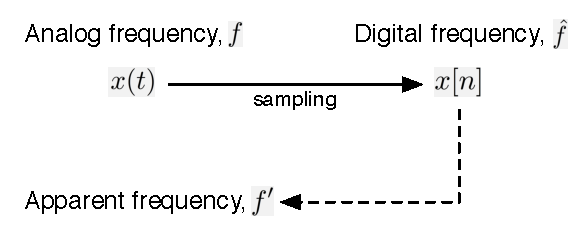
\includegraphics[width=0.7\textwidth]{ch-computer/apparent-frequency}}
  \caption[Sampling and apparent frequency]{Sampling an analog signal,
    $x(t)$, with an analog (actual) frequency $f$ produces a digital
    signal, $x[n]$, at a digital frequency $\hat{f}$. If one examines
    that digital signal and converts $\hat{f}$ back to an analog
    frequency, the apparent frequency is $f'$, which may not be the
    same as $f$, due to aliasing.\label{fg:apparent-frequency}}
\end{figure}

To reconstruct a signal from its samples we need to talk about the
notion of \emph{actual frequency} versus \emph{digital frequency} and
\emph{apparent frequency}, as shown in
figure~\ref{fg:apparent-frequency}. We can use these quantities to
calculate precisely if a frequency will alias, and at what frequency
it will appear. The actual frequency of a signal is the continuous
time frequency that we are accustomed to talking about. For
$e^{j\omega_0 t}$, the actual frequency is $\omega_0$. The digital
frequency is the frequency at which the signal appears to be based on
the indices, $n$, of the sampled signal. Once sampled, $ e^{j\omega_0
  t}$ becomes $ e^{j\omega_0 nT_s}$ which has a digital frequency of
$\hat{\omega}_0=\omega_0 T_s=\omega_0 \frac{2\pi}{\omega_s}$.

\begin{align}
x(t) & = \exp(j\underbrace{\omega_0}_{\stackrel{}{\text{actual}}}t) \notag\\
x[n] & = \exp(j\underbrace{\omega_0 T_s}_{\stackrel{}{\text{digital, $\hat{\omega}$}}} n) \label{eq:samp-phasor-nyq}
\end{align}

Digital frequency, $\hat{\omega}$, \emph{must be} between $-\pi$ and $\pi$. This is because of Nyquist. For example, if the sampling rate, $\omega_s$, is equal to $4\omega_0$, then the digital frequency is
 \[
 \hat{\omega}_0=\omega_0 \times  \frac{2\pi}{\omega_s}=\omega_0\times \frac{2\pi}{4\omega_0}=\frac{\pi}{2} \notag 
 \]
which is less than $\pi$, so Nyquist is satisfied.

Apparent frequency, $\omega'$, is the frequency which we get by
converting from digital frequency back to continuous time
frequency. To convert from digital frequency to apparent we use the
following formula,
\begin{equation}
\omega' = \hat{\omega}\times \frac{\omega_s}{2\pi} \label{eq:conv-dig-app}
\end{equation}
which of course is just the inverse of the previously-used conversion
from continuous to digital frequency.

For our continuing example, when $\omega_s$ is equal to $4\omega_0$,
this means the apparent frequency is $\omega'_0=\pi/2\times
\frac{\omega_s}{2\pi}=\pi/2\times
\frac{4\omega_0}{2\pi}=\omega_0$. Since the sinusoid was sampled at
greater than the Nyquist rate, the apparent frequency equals the
actual frequency.

If we sample at a frequency less than Nyquist the apparent and actual frequencies are different. For example, if we instead sample at $\omega_s=4/3\omega_0$, then the digital frequency will be $\hat{\omega_0}=\omega_0 \frac{2\pi}{4/3\omega_0}=3\pi/2$, which is not on the interval  $-\pi$ to $\pi$. We convert the frequency down by using a clever identity, $e^{-j2\pi n}$, which is equal to 1 for all values of $n$,

\begin{align}
x[n] & = e^{j \frac{3\pi}{2}n} \notag\\
  & = e^{j \frac{3\pi}{2}n} e^{-j2\pi n} && (e^{-j2\pi n}=1)\notag\\
  & = e^{j (\frac{3\pi}{2} -2\pi)n} && (\text{combine exponents})\notag\\
  & = e^{-j \frac{\pi}{2}n} && (\text{equivalent digital frequency}) \notag
\end{align}
%
Essentially, this identity allows us to subtract $2\pi$ from the
digital frequency until it is on the correct interval. Geometrically,
we see that $\frac{3\pi}{2}$ is the same as $-\frac{\pi}{2}$. When we
convert to apparent frequency we get $\omega'_0=-\pi/2\times
\frac{\omega_s}{2\pi}=-\pi/2\times
\frac{4\omega_0}{6\pi}=-\omega_0/3$, which is lesser in magnitude than
the actual frequency and negative (the phasor is spinning in the
opposite direction).

Furthermore, from equation~\ref{eq:conv-dig-app} we can see that the sampling frequency, $\omega_s$, corresponds to the digital frequency $\hat{\omega}=2\pi$. In digital frequency, we have seen that all frequencies at multiples of $2\pi$ from each other have the same apparent frequency. This gives the following relationship between apparent and actual frequency:
 \begin{align}
 \omega'_0 =&\omega_0 + k \omega_s && (k = \ldots, -2, -1, 0, 1, 2, \ldots)
 \end{align}
The apparent frequency could be the result of any frequency that is at a multiple of the sampling frequency. 

%When we sample a function $x(t)$, we get an array $x[n]$ that has no time information (only an index, $n$). Let's assume we sample a signal at a frequency of $\omega_s=2\pi/T_s$ and the signal is a cosine wave at a frequency $\omega_0=\omega_s/4$ (the \emph{actual} frequency is $\omega_0$ and is one fourth the sampling frequency). We know from \ref{eq:samp-phasor} that the discrete signal will be $ \cos{\omega_0 nT_s}$. 
%
%%\begin{align}
%x[n] & = \cos{\omega_0 nT_s}
%     \label{eq:samp-phasor-nyq}
%\end{align}
% 
%Let's explore this in more detail by purposefully sampling
%the signal at too low of a rate. That means that, after sample
%$x[n-1]$ is taken, the next sample --- $x[n]$ --- will be taken some
%number of cycles later. Call the number of cycles between the two
%samples $k$. Clearly, $x[n+1]$ will then occur $k$ cycles after
%$x[n]$, and so on. Since the period of the signal is $2 \pi/\omega_0$,
%we can write the sampling interval as $T'_s = (T_s + k 2
%\pi/\omega_0)$, where $T'_s$ is the sampling interval written to show
%explicitly that it is greater than one cycle of the sinusoid. As in
%equation~(\ref{eq:samp-phasor}), we can write the sampled signal as:
%\begin{align}
%x[n] & = e^{j\omega_0 nT_s} \notag\\
%     &= e^{j\omega_0 nT_s} && \omega_0 = 2/3\omega_s \\
%     &= e^{j2/3\omega_s  nT_s} \\
%x[n] & = e^{j\omega_0 nT'_s} \notag\\
%     & = e^{j\omega_0 n(T_s + k 2 \pi/\omega_0)}
%     &&\text{(substitute expression for cycle skipping, $T'_s$)}
%     \notag\\
%     & = e^{jnT_s(\omega_0 + k 2 \pi/T_s)}
%     &&\text{(factor out $T_s$)}
%     \notag\\
%     & = e^{j\omega'_0 nT_s}
%     &&\text{(where we've called $\omega'_0=\omega_0 + k 2 \pi/T_s$)}
%\label{eq:samp-phasor2}
%\end{align}
%
%By rearranging the terms as in equation~(\ref{eq:samp-phasor2}), we
%see that sampling at too low a rate means that the discrete signal
%$x[n]$ can be interpreted as a phasor with frequency $\omega'_0 =
%\omega_0 + k 2 \pi/T_s$, $k = \ldots, -2, -1, 0, 1, 2, \ldots$.

Now, remember that we are dealing with a real-valued signal, not a
complex-valued one; we use the complex exponential as a representation
that makes the math easier. For a real-valued signal, the imaginary
component of the complex exponential must be canceled out. We can do
this easily by adding another complex exponential at a negative
frequency, since $\cos \omega_0t = 1/2 e^{j\omega_0t} + 1/2
e^{-j\omega_0t}$. So, for a completely real sinusoid we should really write,
\begin{align}
\{\omega'_0\} &= \pm\omega_0 + k\omega_s
\label{eq:set-ambig-freq}
\end{align}

Let's consider the case where $\omega_s/2 < |\omega_0| < \omega_s$,
that is, the sinusoid's frequency is just a bit greater than the
Nyquist frequency (or, equivalently, you could think of it as the
sampling rate being just a bit too slow: $\omega_s <
2|\omega_0|$). Call the amount that $|\omega_0|$ exceeds $\omega_s/2$
$\omega_a = |\omega_0| - \omega_s/2$.  Let's figure out what
happens to the negative frequency component, $-\omega_0$. Using
$\omega_a$, we can rewrite $-\omega_0$ as
\begin{equation}
-\omega_0 = -\omega_a - \omega_s/2
\label{eq:neg-freq}
\end{equation}
(this is simply solving the $\omega_a$ equation for $-\omega_0$).

But we know that, according to equation~(\ref{eq:set-ambig-freq}), the
sinusoid's frequency really corresponds to a set of ambiguous
frequencies, and so we can write equation~(\ref{eq:neg-freq}) as
$-\omega_0 + k\omega_s = -\omega_a - \omega_s/2 + k\omega_s$ to show
\emph{all} of the ambiguous frequencies. To simplify matters, let's
just look at the ``first'' ambiguous frequency at $k=1$:
\begin{align*}
\omega'_0 &= -\omega_0 + \omega_s = -\omega_a- \omega_s/2 + \omega_s
            && (\text{substitute $k=1$}) \\ 
\underbrace{\omega'_0}_{\stackrel{\text{apparent}}{_\text{ frequency}}} &= - \omega_a +
     \underbrace{\omega_s/2}_{\stackrel{\text{Nyquist}}{_\text{ frequency}}}
\end{align*}

So, the apparent frequency is one that is just a bit below the Nyquist
frequency. In fact, if we substitute back in the definition of
$\omega_a$, we get that the apparent frequency is located at $\omega_s
- \omega_0$. So, the first ambiguous frequency for the negative
frequency component of a real sinusoid is located at a positive
frequency.

What if the sampling frequency is not just a bit too slow? In that
case, $\omega_0 > \omega_s$. To find the location of the $k=1$
ambiguous frequency, we can follow the above procedure and find that
we can just subtract multiples of $\omega_s$ from $\omega_0$ until its
absolute value is less than $\omega_s/2$.  Now we can see that the
sampled signal in figure~\ref{fg:sampled} (bottom) must have a frequency of
330-300=30Hz (subtracting the sampling frequency of 300Hz from the
sinusoid's frequency of 330Hz one time).

At the end of chapter~\ref{ch:physical-signals}, we saw how
\emph{any} function can be represented as a sum of sinusoids --- its
Fourier series. If you look at the above discussion, you will see
that, if we replace the phasor in, say,
equation~(\ref{eq:samp-phasor-nyq}) by a sum of phasors at frequencies
$\omega_1, \omega_2, \omega_3, \ldots$, we will reach the same
conclusions, but they will now apply to \emph{each frequency
  component}: each will produce aliases. In the case of the square
wave of Figure~\ref{fig:fs-pulse}, the frequencies of the sinusoids
have no upper limit --- the signal's \emph{spectrum} is infinite.
Certainly, then, there will be frequencies greater than $\omega_s/2$,
regardless of how fast we sample.

How can we avoid this aliasing? We've been discussing the Nyquist
frequency in terms of the sampling frequency; that the signal must
have frequency components less than one-half the sampling frequency.
Another way of looking at sampling is to require that the input signal
be \emph{band limited}: that it have a maximum frequency component,
rather than an infinite spectrum. Given that the signal is band
limited with maximum frequency $\omega_m$ (which we can achieve using
analog \emph{filters}, similar to those described in
chapters~\ref{ch:filt-intro} and~\ref{ch:fb-filters}), then we can set
our sampling rate so that it is at least $2\omega_m$.
\index{analog-to-digital conversion!aliasing|)}

\problemset{
\subsection*{Self-Test Exercises}

See~\ref{sc:ch2ex} \#\ref{it:ch2ex1}--\ref{it:ch2ex3} for answers.

\begin{enumerate}
\item Aliasing can happen in the world around you. Identify the source
  of the original signal and the sampling mechanism in the following
  situations:
\begin{enumerate}
\item The hubcap of a car coming to a stop in a motion picture;
\item A TV news anchor squirming while wearing a tweed jacket;
\item A helicopter blade while the helicopter is starting up on a
  sunny day.
\end{enumerate}
\end{enumerate}
\index{analog-to-digital conversion!sampling|)}}


\section{Quantization}

\index{analog-to-digital conversion!quantization|(}
Understanding aliasing helps us deal with the problems raised by \emph{discretizing time} using
a sample and hold device. There is another discretization that occurs,
however: a discretization of the \emph{analog level} output from the S/H to
the finite number of binary values output by the ADC. This process is
formally known as \emph{quantization}. Since an ideal analog signal
has an infinite number of possible values, while the computer
representation (be it integer or floating point) has a finite number
of values, there will be some error.

\begin{figure}
\centerline{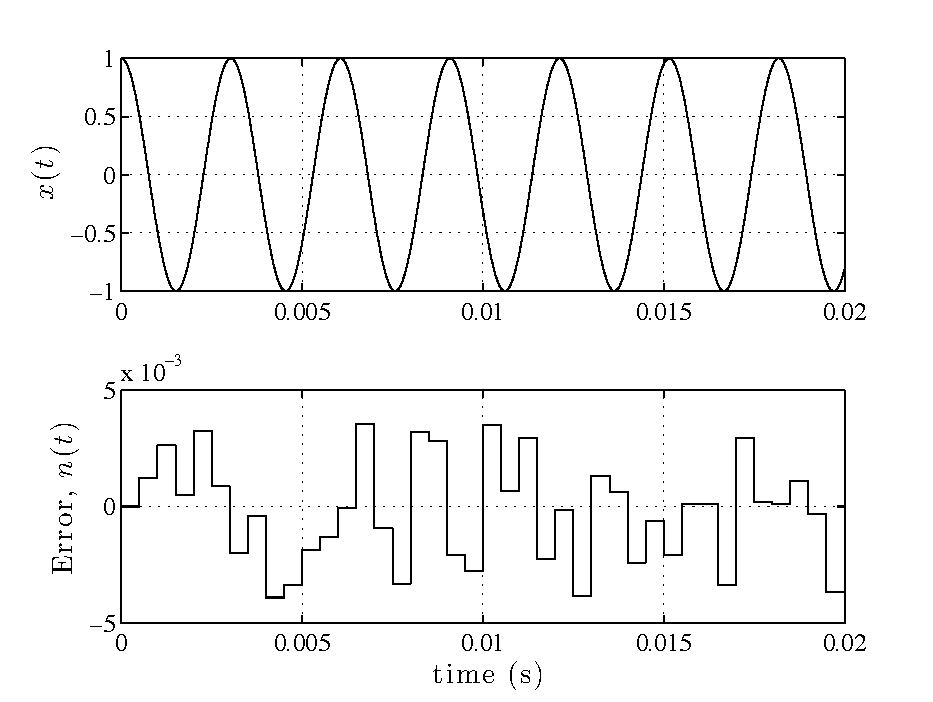
\includegraphics[width=\textwidth]{ch-computer/quant-error_2000}}
\caption[Error in output for 8-bit ADC]{Error in output (bottom) of an
ADC that uses 8 bits to represent values in the range [-1, +1] for the
S/H output in figure~\protect\ref{fg:sampled} (top). Original analog
signal is shown in top plot.\label{fg:quant2k}}
\end{figure}

This error is illustrated in figure~\ref{fg:quant2k}. To produce this
figure, the output of the S/H from figure~\ref{fg:sampled} (top) was
quantized to 256 levels, each corresponding to 1/256 of the distance
between -1 and +1. This result was then subtracted from the ideal S/H
output and plotted as the error shown in the bottom plot in the
figure. How much can this error be? The error can be as much as one
part in $\pm 1/2$ of the least significant bit (LSB). This follows
from the fact that, when we convert the analog value to digital, we
round to the nearest digital number. In other words, the ADC number is
within LSB/2 of the actual signal. What are the statistics of this
noise? Assuming that Nature hasn't conspired against us, we would
expect the mean of this error to be zero.  If all ADC input values
have equal probability, then the errors should also, which means that
it is uniformly distributed between minus and plus one-half.
Remembering our statistics, the standard deviation of a continuous
random variable is the square root of its variance,
\begin{equation}
\sigma^2 = \int_{-\infty}^{+\infty} (x-\mu)^2 \mathrm{d}x
\label{eq:var}
\end{equation}

In this case, $\mu=0$, the variable's range is [-1/2, +1/2], and the
variable's value is constant within that range. The result is a
standard deviation of $\sigma = 1/\sqrt{12} \, \mathrm{LSB} \approx
0.29 \, \mathrm{LSB}$ (how [answer in~\ref{sc:ch2ex}
\#\ref{it:ch2ex4}]?). In the case of an 8-bit ADC, this comes to
0.29/256 = 1/883 of the ADC's full range.

\index{analog-to-digital conversion!quantization!noise|(}
Noise is ubiquitous in the physical world --- and this includes
analog electronics (digital electronics have noise, too, but its
effect on digital signals is different). Sometimes, this noise is
truly random, or \emph{stochastic}, perhaps produced by thermal
effects within the circuitry. Other times, the noise is merely
unwanted signal, such as ``background noise'' in an audio recording.
To quantify this noise we will use SNR (equation \ref{eq:SNR}). The standard deviation, $\sigma$, is an estimate of the noise power ($n_\mathrm{RMS}=\sigma$). For simplicity we will assume that the signal uses the entire ADC range (256 levels, $x_{RMS}=256$).
%Noise is usually quantified as a ratio --- \emph{signal-to-noise
%ratio}, or SNR --- and expressed in decibels (a logarithmic scale). To
%convert a ratio of two magnitudes
%$R_M=\mathrm{Mag}(\mathrm{signal})/\mathrm{Mag}(\mathrm{noise})$ to
%decibels, we calculate
%$\mathrm{SNR_{dB}} = 20 \log_{10}{R_M}$. (If we were talking about a
%ratio of powers $R_P$, it would be $\mathrm{SNR_{dB}} = 10
%\log_{10}{R_P}$.) 
So, for example, if there was no other noise
present than that from quantization by an 8-bit ADC, the SNR would be
$20 \log_{10} 256/0.29 \approx 59\mathrm{dB}$. For a 12-bit ADC, the SNR is
83dB; for 16-bit, the SNR is 107dB.

Another way we might consider the noise that results from quantization
is to consider that amount of noise that it adds given a realistic
signal that already includes other noise. For example, let's suppose
that the ADC input signal has a range of 5 volts (V), and that it
includes noise (from whatever source) with a standard deviation of 1
millivolt (mV). If we use an 8-bit ADC, 5V corresponds to 255 and 1mV
is then 0.051 LSB. (What is the SNR for the original signal (answer
in~\ref{sc:ch2ex} \#\ref{it:ch2ex5}) ?

When we add
random variables, we add their variances, and so the standard
deviation of their sum is the square root of the sum of their
variances, $\sigma' = \sqrt{\sigma_1^2 + \sigma_2^2}$. For an 8-bit
ADC, then, we have the total noise (inherent plus quantization) of
$\sqrt{0.051^2 + 0.29^2} = 0.294 \, \textrm{LSB}$. So, almost all of
the noise in the digitized signal is caused by quantization (the noise
on the output represents a 476\% increase from the input noise)! If we
go to 12 bits, the total noise is $\sqrt{0.82^2 + 0.29^2} = 0.87 \,
\textrm{LSB}$ --- quantization increases the noise by 6\%. From a
design point of view, we \emph{select} the ADC based in part on the
expected noise in the analog signal and the maximum noise we can
tolerate in the digital one.  \index{analog-to-digital
  conversion!quantization!noise|)}

\problemset{
\subsubsection*{MATLAB and Sound Files}
\begin{sloppypar}
\begin{itemize}
\item A MATLAB .m file for demonstrating quantization using tones is available
at \url{http://faculty.washington.edu/stiber/pubs/Signal-Computing/quantdemo1.m}.
\index{MATLAB code!quantization}
\item A MATLAB .m file for demonstrating quantization using a more
interesting sound is available at
\url{http://faculty.washington.edu/stiber/pubs/Signal-Computing/quantdemo2.m},
\index{MATLAB code!quantization}
along with a data file at
\url{http://faculty.washington.edu/stiber/pubs/Signal-Computing/amoriole2.mat}.
\index{audio files!bird calls}
\end{itemize}
\end{sloppypar}}

\problemset{
\subsection*{Self-Test Exercises}

See~\ref{sc:ch2ex} \#\ref{it:ch2ex6} for the answer.

\begin{enumerate}
\item What ratio of amplitudes is represented by one bel?
\end{enumerate}
\index{analog-to-digital conversion!quantization|)}}

\section{Dynamic Range}

\index{analog-to-digital conversion!dynamic range|(}
So, one reason we might choose an ADC with more bits is to reduce the
effects of quantization noise.  There is another reason: our desire to
represent both low and high amplitude signals with reasonable
fidelity. The need for this \emph{dynamic range} can result in us
needing more bits.  Let's use as an example the digitization of an
orchestra where the ratio of the low amplitude passages to the high
amplitude ones is 1/1000 (60dB).  If we use an 8-bit ADC, then 255
corresponds to the highest amplitude and the lowest amplitude is 0.255
LSB. In other words, we have used just about all the bits for the
loudest passages, leaving nothing for the quiet parts!  For a 12-bit
ADC, the lowest amplitudes are allocated about 2 bits; for a 16-bit
ADC, only about 6 bits. The reason for this is that we've coded the
signal \emph{linearly}, with the step between ADC outputs being the
same for low and high amplitude signals. Logically, however, it would
seem unlikely that our ears would be as sensitive to slight changes in
loud passages as they would be to the same changes to quiet ones ---
that at least some part of our perception would be based on relative
comparisons, not just absolute differences.

This intuition is correct, and so consideration of the
\emph{psychophysics} of hearing (the intersection of the physics of
sound and the psychology of perception) leads us to a solution for
\index{perception!auditory!psychophysics}
audio digitization: \emph{companding}. 
\index{companding}
We first pass the analog signal through a ``squashing function''
before digitization. This nonlinear function doesn't modify the quiet
passages (the region of the function near zero is basically linear,
with a slope of one).  However, it causes changes in loud passages to
result in smaller changes in the signal to be digitized. This is
equivalent to allocating more bits to the quiet passages and fewer to
the loud ones. Assuming we use the exact inverse function on any audio
output provided by our system, there should be little noticeable
effect of this companding.

Of course, this is all based on the assumption that we are digitizing
a signal that will be listened to. If, on the other hand, the signal
is some other kind of data not for ``human consumption,'' then small
steps at high amplitude may be just as important as those at low ones,
and so companding won't be usable --- it would destroy valuable
information.
\index{analog-to-digital conversion!dynamic range|)}
\index{analog-to-digital conversion|)}

\section{Periodic and Aperiodic Signals}

In this chapter, we talked about a signal as being a sum of sinusoids,
as in chapter~\ref{ch:physical-signals}. In general, a periodic
signal can be expressed as a sum of \emph{both} sines and cosines,
which we can express as the sum of complex sinusoids:
\begin{equation}
f(t) = \sum_{k=-\infty}^{+\infty} c_k e^{jk 2\pi t/T}
\label{eq:fseries}
\end{equation}

Equation~(\ref{eq:fseries}) is the general Fourier series, which can
be used to represent any periodic signal with period $T$. In this
series, all of the complex sinusoids have periods that are multiples
of $T$ (frequencies that are multiples of $2\pi/T$). So, the frequency
content, or \emph{spectrum}, of a periodic signal (the $c_k$s) is
\emph{discrete}: it only has values at particular frequencies.

As we shall see in chapter~\ref{ch:fft}, for an aperiodic signal, the
Fourier series becomes the \emph{Fourier integral}, and the signal's
spectrum is \emph{continuous}:
\begin{equation}
f(t) = \frac{1}{2\pi} \int_{-\infty}^{+\infty} F(j\omega)
                          e^{j\omega t} \mathrm{d}\omega
\label{eq:fint}
\end{equation}

In equation~(\ref{eq:fint}), the function $F(j\omega)$ describes the
magnitude of the complex sinusoid at frequency $\omega$.  This is the
continuous (because $\omega$ can take on all values, not just a
discrete set) spectrum of an aperiodic signal. Intuitively, we take the limit as the period of the signal goes to infinity in equation~\ref{eq:fseries}, which pushes the spacing between the $c_k$ spectral lines closer and closer until the spectrum becomes continuous. I'll revisit this
topic later, in more detail.

\section{Problems}

%\begin{enumerate}
%\item The analytical formula for synthesis of a 50\% duty cycle square
%  wave as a sum of harmonically related sine waves (its Fourier
%  series) is:
%  \begin{equation*}
%    x(t) = \frac{4}{\pi} \left( \sin(\omega_0 t)
%      + \frac{1}{3} \sin(3\omega_0 t)
%      + \frac{1}{5} \sin(5\omega_0 t) + \cdots \right)
%  \end{equation*}
%  Write a MATLAB program to compute and plot the spectrum of a square
%  wave given this equation.  Your program should prompt the user for
%  $\omega_0$ and which harmonic is the maximum to plot. Note that you
%  are \emph{not} being asked to plot the square wave as a function of
%  time; you should plot the amplitudes of the component sinusoids as a
%  function of the sinusoids' frequencies (like
%  figure~\ref{fig:fs-pulsecn}). Hand in hard copy of your MATLAB code
%  and a plot of the spectrum with 10 harmonics. You may find the
%  MATLAB function \texttt{stem()} useful.\label{it:sq-wave-spectrum}
%
%\item Modify your above program to show how these harmonics are
%  aliased if the square wave is sampled at $\omega_s$ (prompting the
%  user for $\omega_s$). Hand in hard copy of your code and an example
%  plot for $\omega_s < \omega_0$.\label{it:aliased-sq-wave}
%
%\item Modify your program to play the sound of the aliased square wave
%  (synthesize $x(t)$ from problem~\ref{it:aliased-sq-wave}). Next,
%  write a program to generate a band-limited square wave from a sum of
%  sinusoids, given $\omega_0$ and $\omega_s$, with no frequency
%  components above the Nyquist limit. Play that sound (the MATLAB
%  function \texttt{soundsc()} is useful for this). Compare the sounds
%  with and without (from problem~\ref{it:sq-wave-spectrum}, given that
%  $\omega_s$ determines $\omega_\mathit{max}$) aliasing. Can you find
%  an interesting use for intentional aliasing? Hand in your code's
%  hard copy, plots of the sample square wave and the band limited
%  square wave (as functions of \emph{time}), and your written
%  comments.
%\end{enumerate}

\begin{enumerate}

\item What is the RMS magnitude of the sine wave $A\sin(\omega t)$?

\item What is the RMS magnitude of the sawtooth waveform 
\begin{equation*}
			x(t) = \frac{A}{T} t\text{,        } 0<t<=T
\end{equation*}
			where $x(t)$ repeats every $T$ seconds

\item The sin wave from problem 1 is sampled in noise, 
			if the desired SNR is 20 dB, how large can the RMS magnitude of the noise be?

\item If the sawtooth waveform from problem 2 is considered noise and
			the sine wave from problem 1 is the signal, what is the SNR in dB?

\item The signal $e^{j 2\pi \times200 t}$ is sampled at $\omega_s=2\pi\times300$. 
			What are the actual, digital, and apparent frequencies?

\item The signal $\cos( 2\pi \times200 t)$ is sampled at $\omega_s=2\pi\times250$.
			What are the actual, digital and apparent frequencies of the resulting cosines?

\item Consider the 50\% duty cycle square wave with amplitude from -1 to 1 and period $T$.
\begin{enumerate}
\item What is the RMS magnitude?
\item The fourier series of the 50\% duty cycle square wave is given by,
\begin{equation*}
\frac{4}{\pi} \sum_{k=1,3,5...}^\infty \frac{\sin(k \omega_0 t)}{k}
\end{equation*}			
If we consider the ``band limit'' of the square wave to be when it has no other frequencies with magnitudes larger than 1\% of the RMS magnitude, then what is the minimum sampling rate to capture all frequencies below the ``band limit'' without aliasing?
	\end{enumerate}
\item Suppose we wish to sample from an audio signal that ranges from 0 to 2.5V (Assume that the range of our ADC is 0-2.5V also). If the analog noise on the line is 3mV and our ADC is 8bits, what percentage of the total SNR is from the analog noise and what percentage is from the 8 bit quantization?
\item If we have the same signal from question 8 (audio signal from 0-2.5V with 3mV analog noise), 
	\begin{enumerate}
			\item how many bits should our ADC have so that the noise added by quantization is less than the analog noise?
			\item how many bits should our ADC have so that the quantization noise does not decrease our SNR by more than 1\%?
	\end{enumerate}

\end{enumerate}

\section{Further Reading}

James H McClellan, Ronald W. Schafer, and Mark A. Yoder, \textit{DSP
  First: A Multimedia Approach}, Prentice Hall, 1998, chapter 4 (\S
4.1--4.3).

% LocalWords:  phasors
